\section{Resultados e discussão}\label{sec:resultados}

Esta seção apresenta os resultados obtidos com a plataforma computacional descrita na Seção~\ref{sec:metodologia}, aplicada a uma matriz de configurações de ponte de madeira roliça para estrada vicinal de pista simples.
A matriz combina quatro vãos teóricos com as cinco classes de resistência de madeiras de florestas nativas da ABNT NBR 7190-3, mantendo fixos a largura da pista, o trem tipo e todos os coeficientes normativos, de modo que as diferenças observadas decorram exclusivamente do vão e da classe de resistência.

A apresentação está organizada em três blocos.
O primeiro descreve a plataforma computacional desenvolvida (Seção~\ref{sec:plataforma}) e define a matriz de casos (Seção~\ref{sec:casos}).
O segundo detalha exaustivamente uma célula de referência da matriz (Seção~\ref{sec:caso_detalhado}), na qual são exercitados todos os recursos analíticos da ferramenta: fronteira eficiente, grau de utilização das verificações, custo da robustez, convergência por hipervolume, sensibilidade global de Sobol e dispersão das variáveis de projeto.
O terceiro percorre a matriz completa (Seção~\ref{sec:varredura}) e converte os resultados em ábacos de anteprojeto (Seção~\ref{sec:abacos}).


\subsection{Plataforma computacional}\label{sec:plataforma}

Como principal produto de engenharia deste trabalho, foi desenvolvida uma plataforma computacional de acesso livre para o dimensionamento de pontes de madeira, capaz de realizar a verificação completa dos elementos estruturais em conformidade com as ABNT NBR 7190 \parencite{NBR7190-1:2022} e NBR 7188 \parencite{nbr7188}, disponível nos idiomas português e inglês \parencite{ReliaBridge2026}.
A interface, ilustrada nas Figuras~\ref{fig:tela_inicial} e~\ref{fig:interface_dim}, é organizada em módulos que permitem a navegação sequencial entre as etapas de dimensionamento por otimização, projeto detalhado dos elementos e análise dos resultados.
Ao final do processamento, a ferramenta disponibiliza para download a planilha de dados de entrada, os resultados do pré-dimensionamento, as estatísticas descritivas das variáveis de projeto e as figuras geradas.

\begin{figure}[!ht]
    \centering
    
\includegraphics[width=0.85\textwidth]{figuras/inicio.png}
    \caption{Tela inicial da plataforma computacional.}
    \label{fig:tela_inicial}
\end{figure}

\begin{figure}[!ht]
    \centering
    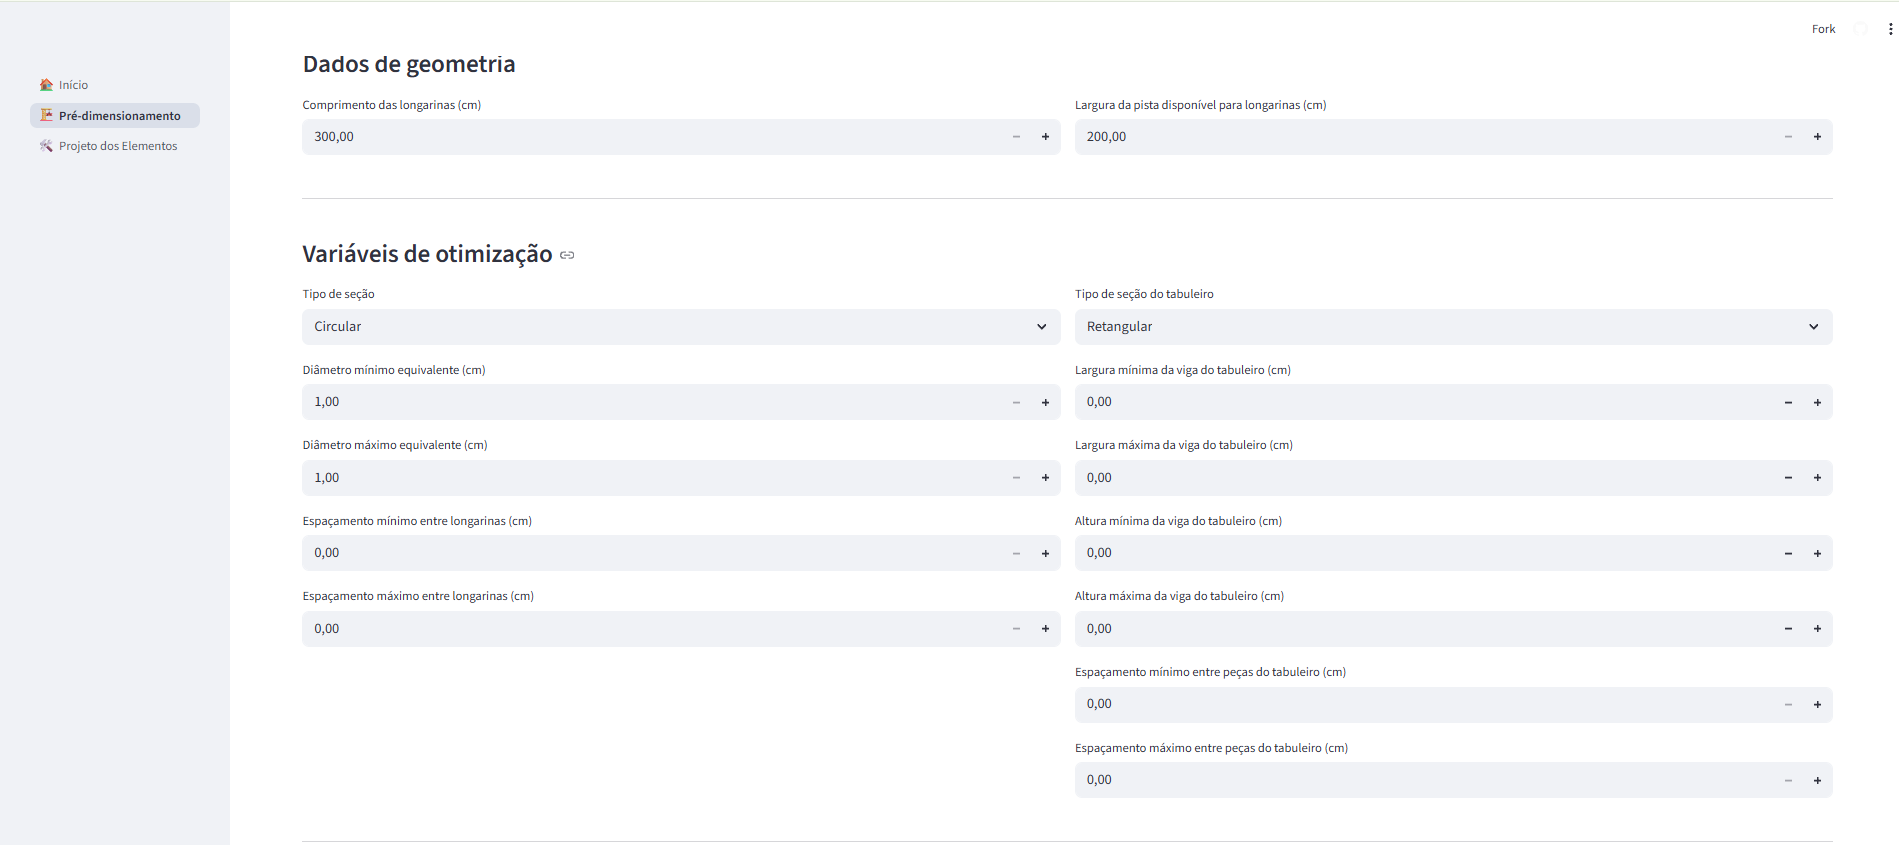
\includegraphics[width=0.9\textwidth]{figuras/predimencionamento.png}
    \caption{Módulo de dimensionamento por otimização.}
    \label{fig:interface_dim}
\end{figure}

\subsection{Definição da matriz de casos de estudo}\label{sec:casos}

Os parâmetros geométricos, de carregamento e os coeficientes normativos mantidos constantes em toda a matriz são apresentados na Tabela~\ref{tab:parametros}.
A largura de pista de 4{,}5~m corresponde à seção transversal usual de ponte vicinal de pista simples, compatível com o tráfego de um veículo por vez e com guarda-rodas laterais.

\begin{table}[!ht]
\caption{Parâmetros geométricos, de carregamento e coeficientes normativos comuns a toda a matriz.\label{tab:parametros}}
\begin{threeparttable}
\begin{tabular*}{\columnwidth}{@{\extracolsep\fill}lc@{\extracolsep\fill}}
\toprule
Parâmetro & Valor \\
\midrule
Largura da pista, $b_{w,\mathrm{pista}}$ (cm) & 450 \\
Trem tipo (ABNT NBR 7188) & TB-240 \\
Carga concentrada por roda, $p_{rodak}$ (kN) & 40 \\
Carga variável distribuída, $p_{qk}$ (kPa) & 4 \\
Carga permanente distribuída (rodeiro), $p_{gk}$ (kPa)\tnote{a} & 0{,}10 \\
Distância entre eixos, $a$ (m) & 1{,}5 \\
Classe de carregamento & Curta duração \\
Classe da madeira & Madeira natural \\
Classe de umidade & 3 \\
Coeficiente parcial das ações permanentes, $\gamma_g$ & 1{,}30 \\
Coeficiente parcial das ações variáveis, $\gamma_q$ & 1{,}50 \\
Coeficiente de minoração (tensões normais), $\gamma_{wf}$ & 1{,}40 \\
Coeficiente de minoração (cisalhamento), $\gamma_{wc}$ & 1{,}80 \\
Fator de combinação quase permanente, $\psi_2$ & 0{,}30 \\
Coeficiente de fluência, $\varphi$ & 0{,}80 \\
Desvio de robustez, $\rho$ (\%) & 5{,}0 \\
\bottomrule
\end{tabular*}
\begin{tablenotes}
\footnotesize
\item[a] O peso próprio do tabuleiro e das longarinas é calculado internamente pela plataforma a partir da geometria e da densidade da madeira. A carga permanente $p_{gk}$ representa apenas a ação sobreposta do rodeiro, isto é, das tábuas longitudinais de rolamento que guiam as rodas.
Estimou-se essa parcela a partir de duas tábuas de seção $5 \times 30$~cm, com densidade de 620~kg/m\textsuperscript{3} ($\gamma \approx 6{,}1$~kN/m\textsuperscript{3}), resultando em cerca de 0{,}18~kN/m ao longo do vão, ou aproximadamente 0{,}04~kPa quando distribuída sobre a largura da pista.
Adotou-se o valor de 0{,}10~kPa, arredondado para cobrir fixações e a maior densidade usual das peças de rolamento.
\item As propriedades mecânicas da madeira não constam desta tabela por variarem entre as células da matriz. São as da Tabela~\ref{tab:classes_madeira}, conforme a classe de resistência de cada célula.
\end{tablenotes}
\end{threeparttable}
\end{table}

A matriz de casos é o produto cartesiano de quatro vãos teóricos por cinco classes de resistência, totalizando vinte configurações, conforme a Tabela~\ref{tab:matriz}.
A faixa de vãos de 3{,}0 a 6{,}0~m foi escolhida por dois motivos.
O primeiro é de representatividade: corresponde à extensão usual dos cursos d'água transpostos por pontes de madeira roliça em vias vicinais.
O segundo é de consistência de formulação: nesse intervalo o momento fletor devido à carga móvel é dado integralmente pela Equação~\eqref{eq:mqk30}, sem a parcela adicional de multidão da Equação~\eqref{eq:mqk45}, de modo que as curvas de resultado não apresentam descontinuidade de formulação.

\begin{table}[!ht]
\caption{Matriz de casos de estudo. Cada célula corresponde a uma execução independente do NSGA-II.\label{tab:matriz}}
\begin{threeparttable}
\begin{tabular*}{\columnwidth}{@{\extracolsep\fill}lccccc@{\extracolsep\fill}}
\toprule
 & \multicolumn{5}{c}{Classe de resistência (ABNT NBR 7190-3)} \\
\cmidrule{2-6}
Vão $L$ (m) & D20 & D30 & D40 & D50 & D60 \\
\midrule
3{,}0 & C-01 & C-02 & C-03 & C-04 & C-05 \\
4{,}0 & C-06 & C-07 & C-08 & C-09 & C-10 \\
5{,}0 & C-11 & C-12 & \textbf{C-13} & C-14 & C-15 \\
6{,}0 & C-16 & C-17 & C-18 & C-19 & C-20 \\
\bottomrule
\end{tabular*}
\begin{tablenotes}
\footnotesize
\item A célula C-13 ($L = 5{,}0$~m, classe D40), destacada em negrito, é adotada como caso de referência para a análise detalhada da Seção~\ref{sec:caso_detalhado}.
\end{tablenotes}
\end{threeparttable}
\end{table}

Os intervalos de busca das cinco variáveis de projeto, comuns a todas as células, são apresentados na Tabela~\ref{tab:intervalos}.
Os limites foram estabelecidos de modo a abranger as dimensões comerciais usuais de madeira roliça e de pranchas serradas, sem restringir artificialmente o espaço de busca do algoritmo.

\begin{table}[!ht]
\caption{Intervalos adotados para as variáveis de projeto.\label{tab:intervalos}}
\begin{threeparttable}
\begin{tabular*}{\columnwidth}{@{\extracolsep\fill}lcc@{\extracolsep\fill}}
\toprule
Variável & Valor mínimo (cm) & Valor máximo (cm) \\
\midrule
Diâmetro da longarina, $d$ & 30 & 150 \\
Largura da prancha do tabuleiro, $b_w$ & 5 & 60 \\
Altura da prancha do tabuleiro, $h$ & 5 & 60 \\
Espaçamento entre longarinas, $esp_{long}$ & 30 & 200 \\
Espaçamento entre peças do tabuleiro, $esp_{tab}$ & 2 & 5 \\
\bottomrule
\end{tabular*}
\end{threeparttable}
\end{table}

\subsection{Caso de referência detalhado: $L = 5{,}0$~m, classe D40}\label{sec:caso_detalhado}

Esta seção exercita todos os recursos analíticos da plataforma sobre uma única célula da matriz, a C-13.
A escolha recai sobre um vão intermediário e uma classe de resistência intermediária, de modo que o comportamento observado seja representativo do conjunto.
Os resultados das demais dezenove células são reportados de forma condensada na Seção~\ref{sec:varredura}.

\subsubsection{Fronteira eficiente e soluções representativas}\label{sec:fronteira_ref}

A otimização robusta multiobjetivo da célula C-13, com $\rho = 5\%$, gerou um conjunto de soluções não dominadas distribuídas ao longo da fronteira eficiente, apresentada na Figura~\ref{fig:fronteira_ref}.
A Tabela~\ref{tab:solucoes_ref} reúne uma amostra representativa dessas soluções, com as respectivas funções objetivo e o maior valor entre as seis funções limite, confirmando o atendimento aos critérios normativos mesmo sob a avaliação robusta.

\begin{figure}[!ht]
    \centering
    
\includegraphics[width=0.6\textwidth]{figuras/pareto_frontier_C13.png}
    \caption{Fronteira eficiente da célula de referência C-13 ($L = 5{,}0$~m, D40, $\rho = 5\%$).}
    \label{fig:fronteira_ref}
\end{figure}

\begin{table}[!ht]
\caption{Soluções representativas da fronteira eficiente da célula C-13.\label{tab:solucoes_ref}}
\begin{threeparttable}
\setlength{\tabcolsep}{3pt}
\begin{tabular*}{\textwidth}{@{\extracolsep{\fill}}cccccccc@{\extracolsep{\fill}}}
\toprule
$d$ (cm) & $b_w$ (cm) & $h$ (cm) & $esp_{long}$ (cm) & $esp_{tab}$ (cm) & $V_{\mathrm{total}}$ (m\textsuperscript{3}) & $\delta_{\mathrm{tot}}/(L/350)$ & $g_{\max}$ \\
\midrule
45{,}71 & 46{,}51 & 7{,}51 & 103{,}58 & 2{,}26 & 4{,}83 & 0{,}3355 & $-0{,}0000$ \\
49{,}51 & 46{,}96 & 7{,}17 & 99{,}82 & 2{,}35 & 5{,}33 & 0{,}2476 & $-0{,}0367$ \\
55{,}84 & 47{,}55 & 11{,}18 & 132{,}81 & 2{,}84 & 5{,}99 & 0{,}1698 & $-0{,}0335$ \\
67{,}09 & 46{,}21 & 10{,}17 & 108{,}48 & 2{,}35 & 7{,}39 & 0{,}0855 & $-0{,}0097$ \\
85{,}04 & 47{,}93 & 9{,}64 & 106{,}05 & 3{,}15 & 10{,}48 & 0{,}0368 & $-0{,}2940$ \\
110{,}59 & 46{,}07 & 5{,}09 & 124{,}80 & 2{,}84 & 15{,}37 & 0{,}0152 & $-0{,}2664$ \\
150{,}00 & 46{,}51 & 11{,}82 & 136{,}09 & 2{,}61 & 20{,}01 & 0{,}0065 & $-0{,}0279$ \\
\bottomrule
\end{tabular*}
\begin{tablenotes}
\footnotesize
\item Sete soluções extraídas da fronteira final de 50 pontos não dominados, ordenadas do extremo de menor volume de madeira (primeira linha) ao extremo de menor flecha adimensional (última linha), incluindo ambos os extremos. $g_{\max}$ é o maior valor entre as funções limite de resistência e de serviço $g_1$ a $g_4$ da solução, e é negativo em todas as linhas, o que confirma a viabilidade sob a avaliação robusta.
As funções limite geométricas $g_5$ e $g_6$, que apenas verificam o enquadramento dos espaçamentos nos intervalos da Tabela~\ref{tab:intervalos}, não entram nesse máximo por não expressarem margem estrutural.
\end{tablenotes}
\end{threeparttable}
\end{table}

A fronteira estende-se de 4{,}83~m\textsuperscript{3} de madeira, com flecha total igual a 33{,}6\% do limite normativo, até 20{,}01~m\textsuperscript{3}, com flecha de apenas 0{,}65\% do limite.
Os dois objetivos variam, portanto, em escalas muito distintas: enquanto o volume pouco mais que quadruplica, a flecha adimensional cai cerca de cinquenta vezes.
Esse desequilíbrio é a manifestação direta da geometria da seção circular.
O volume cresce aproximadamente com $d^{1{,}22}$ ao longo da fronteira, ao passo que a flecha decresce com $d^{-3{,}37}$, de modo que o ajuste conjunto resulta em $\delta_{\mathrm{tot}}/(L/350) \propto V^{-2{,}74}$, com coeficiente de determinação de 0{,}997.
Em termos de projeto, isso significa que os primeiros metros cúbicos adicionais de madeira compram uma redução expressiva de deslocamento: dobrar o volume a partir do extremo econômico já reduz a flecha em cerca de oito vezes, e dobrá-lo novamente reduz esse valor por um fator adicional de aproximadamente seis. O retorno, contudo, deixa de ter relevância prática nesse segundo intervalo, pois a flecha já está bem abaixo de 1\% do limite normativo desde o primeiro dobramento.
O trecho útil da fronteira para o projetista concentra-se, assim, no primeiro terço da curva.

A restrição ativa ao longo da fronteira é a mesma em todos os pontos analisados.
A flexão do tabuleiro ($g_4$) é a verificação mais próxima do limite nas 50 soluções da fronteira, inclusive no extremo de menor volume, onde satura exatamente no limite normativo ($g_{\max} \approx 0$, utilização de 100{,}0\%).
A flexão da longarina ($g_1$) acompanha de perto nesse mesmo extremo, com utilização de 99{,}7\%, mas sem nunca ultrapassar o tabuleiro como restrição governante ao longo da fronteira.
A leitura de projeto que decorre disso é relevante: percorrer a fronteira significa engrossar a longarina, que rapidamente ganha folga, ao passo que o tabuleiro permanece encostado no seu limite ao longo de todo o espaço de compromisso.
O tabuleiro, portanto, não é um elemento secundário do dimensionamento: é o elemento que limita o desempenho. O par largura-altura da prancha e o espaçamento entre longarinas definem o vão de flexão local sob a roda, e são eles que ditam a forma da curva da Figura~\ref{fig:fronteira_ref}.

\subsubsection{Grau de utilização das verificações normativas}\label{sec:utilizacao}

A Figura~\ref{fig:utilizacao} apresenta o grau de utilização de cada verificação normativa para uma solução selecionada da fronteira, entendido como a razão entre solicitação e resistência, no caso dos estados limites últimos, ou entre deslocamento e limite admissível, no caso do estado limite de serviço.
O valor de 100\% corresponde ao limite normativo.
Como as funções limite são normalizadas na forma $g_j = (S_j - R_j)/R_j$, o grau de utilização decorre diretamente delas por $(1 + g_j)\times 100\%$.
A solução analisada é a de menor volume de madeira da fronteira, primeira linha da Tabela~\ref{tab:solucoes_ref}, por ser a de interesse imediato para o anteprojeto.
Essa figura complementa a demonstração manual de verificação apresentada no Apêndice~\ref{ap:demonstracao}.

\begin{figure}[!ht]
    \centering
    
\includegraphics[width=0.75\textwidth]{figuras/utilizacao_C13.png}
    \caption{Grau de utilização de cada verificação normativa para a solução selecionada da fronteira robusta da célula C-13.}
    \label{fig:utilizacao}
\end{figure}

A solução econômica da célula C-13 apresenta duas verificações praticamente saturadas e duas com folga apreciável.
A flexão do tabuleiro governa o dimensionamento, com utilização de 100{,}0\%, valor consistente com o $g_{\max} \approx 0$ registrado na primeira linha da Tabela~\ref{tab:solucoes_ref}.
Imediatamente atrás vem a flexão da longarina, a 99{,}7\%.
As duas verificações de flexão, portanto, tornam-se ativas quase simultaneamente, o que é a assinatura de um dimensionamento bem equilibrado: o algoritmo não pôde reduzir mais o volume porque teria de violar uma das duas ao mesmo tempo em que a outra ainda estava no limite.

As folgas concentram-se nas verificações restantes.
A flecha da longarina opera a 73{,}2\% do deslocamento limite $L/350$ e o cisalhamento a 45{,}0\% da resistência de cálculo, sendo esta última a verificação com maior reserva.
O resultado tem consequência prática direta: no vão de 5~m, para a madeira D40 e o trem tipo TB-240, o dimensionamento é integralmente controlado por resistência à flexão, e não por rigidez.
A ampla folga ao cisalhamento decorre da geometria circular, na qual a área da seção cresce com $d^2$ enquanto a solicitação de cortante independe do diâmetro, e indica que a verificação ao esforço cortante, tradicionalmente citada como crítica em peças roliças curtas, não é determinante nesta faixa de vãos.

\subsubsection{Custo da robustez}\label{sec:custo_robustez}

A otimização determinística tende a posicionar as soluções ótimas exatamente sobre a fronteira das restrições ativas, tornando-as sensíveis a pequenas variações nas variáveis de projeto.
Em pontes de madeira roliça, essa sensibilidade é agravada pela variabilidade natural do diâmetro das peças e pelas tolerâncias de fabricação e montagem.
A incorporação da robustez desloca a fronteira eficiente para o interior do domínio viável: enquanto a otimização determinística tende a produzir soluções com função limite de flexão da longarina praticamente nula ($g_1 \approx 0$), a otimização robusta penaliza essas soluções, pois sob perturbação de $\pm\rho$ parte das realizações resultaria em violação.

Para quantificar esse efeito, a célula C-13 foi reotimizada para quatro níveis de desvio, $\rho \in \{0\%,\ 2{,}5\%,\ 5\%,\ 10\%\}$, mantendo inalterados todos os demais parâmetros do algoritmo (Tabela~\ref{tab:nsga2}).
O caso $\rho = 0\%$ corresponde à otimização determinística, com $N_c = 1$, e serve de referência.

\begin{figure}[!ht]
    \centering
    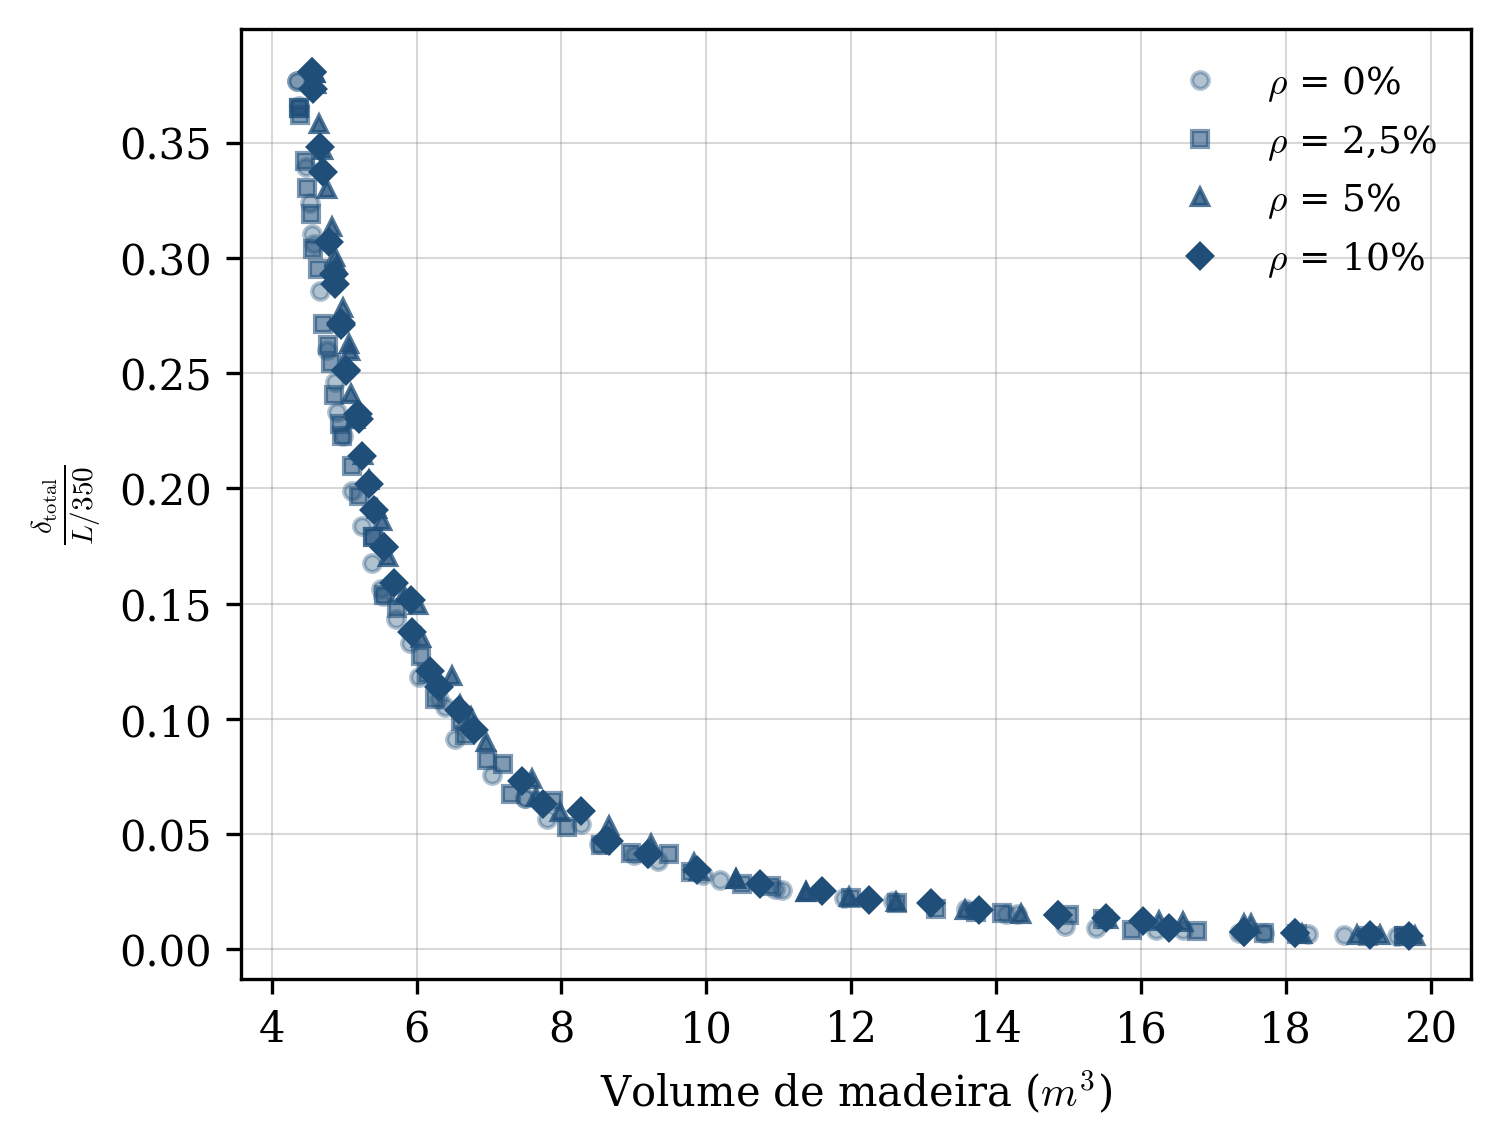
\includegraphics[width=0.7\textwidth]{figuras/custo_robustez_C13.png}
    \caption{Fronteiras eficientes da célula C-13 para $\rho = 0\%$, $2{,}5\%$, $5\%$ e $10\%$.}
    \label{fig:custo_robustez}
\end{figure}

\begin{table}[!ht]
\caption{Acréscimo percentual de volume de madeira em relação ao caso determinístico ($\rho = 0\%$), para três níveis pareados de flecha adimensional.\label{tab:custo_robustez}}
\begin{threeparttable}
\setlength{\tabcolsep}{3pt}
\begin{tabular*}{\columnwidth}{@{\extracolsep\fill}lccccccc@{\extracolsep\fill}}
\toprule
$\delta_{\mathrm{tot}}/(L/350)$ & $V(0\%)$ & $V(2{,}5\%)$ & $\Delta$ & $V(5\%)$ & $\Delta$ & $V(10\%)$ & $\Delta$ \\
\midrule
0{,}0500 & 8{,}391 & 8{,}267 & $-1{,}5\%$ & 8{,}915 & $+6{,}2\%$ & 8{,}544 & $+1{,}8\%$ \\
0{,}1000 & 6{,}445 & 6{,}577 & $+2{,}0\%$ & 6{,}762 & $+4{,}9\%$ & 6{,}677 & $+3{,}6\%$ \\
0{,}1500 & 5{,}599 & 5{,}672 & $+1{,}3\%$ & 5{,}982 & $+6{,}8\%$ & 5{,}930 & $+5{,}9\%$ \\
\bottomrule
\end{tabular*}
\begin{tablenotes}
\footnotesize
\item Volume em m\textsuperscript{3}. $\Delta$ é o acréscimo percentual em relação a $V(0\%)$ para o mesmo nível de flecha adimensional.
\end{tablenotes}
\end{threeparttable}
\end{table}

A Figura~\ref{fig:custo_robustez} mostra as quatro fronteiras praticamente sobrepostas na região de maior volume, onde a folga já é ampla o bastante para absorver a perturbação, e progressivamente separadas rumo ao extremo de menor volume, onde a restrição de flexão da longarina está mais próxima do limite.
É nesse extremo que a robustez tem efeito prático: a solução de menor volume desloca-se de 4{,}347~m\textsuperscript{3} em $\rho = 0\%$ para 4{,}380~m\textsuperscript{3} ($+0{,}8\%$) em $\rho = 2{,}5\%$, 4{,}599~m\textsuperscript{3} ($+5{,}8\%$) em $\rho = 5\%$ e 4{,}560~m\textsuperscript{3} ($+4{,}9\%$) em $\rho = 10\%$.

O deslocamento da fronteira não é estritamente monotônico ponto a ponto: a Tabela~\ref{tab:custo_robustez} registra $\Delta$ negativo para $\rho = 2{,}5\%$ no nível de flecha mais próximo do extremo econômico (0,0500). O mesmo efeito aparece, de forma mais visível, tanto no extremo econômico da fronteira quanto na média pareada dos três níveis de flecha: o acréscimo médio de volume é de $+0{,}6\%$ em $\rho = 2{,}5\%$, $+6{,}0\%$ em $\rho = 5\%$ e $+3{,}8\%$ em $\rho = 10\%$, ou seja, o valor registrado em $\rho = 10\%$ é inferior ao de $\rho = 5\%$ em ambos os indicadores. Isso é esperado, pois $\rho = 0\%$, $2{,}5\%$, $5\%$ e $10\%$ são execuções independentes e únicas do NSGA-II, sem repetição de semente por nível, e diferenças dessa ordem de grandeza estão dentro do ruído de convergência do algoritmo entre execuções, não de um efeito físico de sinal trocado.
A leitura mais conservadora, e a que este trabalho adota, é a de que o custo da robustez cresce de forma consistente entre $\rho = 0\%$ e $\rho = 5\%$ e, a partir daí, estabiliza em um patamar da ordem de 4\% a 6\% de material adicional: nestes dados, dobrar a tolerância de $\rho = 5\%$ para $\rho = 10\%$ não produz agravamento adicional mensurável, seja para uma solução de compromisso, seja para o extremo mais econômico da fronteira.

As quatro execuções, rodadas sequencialmente na mesma máquina, consumiram 7{,}2~s ($\rho = 0\%$), 18{,}7~s ($\rho = 2{,}5\%$), 18{,}7~s ($\rho = 5\%$) e 18{,}5~s ($\rho = 10\%$) de processamento.
A diferença entre o caso determinístico e os demais decorre integralmente de $N_c$ colapsar para uma única avaliação quando $\rho = 0$ (Seção~\ref{sec:robustez}), contra as $N_c = 30$ avaliações perturbadas por indivíduo nos demais níveis: uma vez ativado o mecanismo de robustez, o tempo de processamento é praticamente insensível à magnitude de $\rho$, consistente com o custo computacional escalar com o número de avaliações perturbadas por indivíduo, e não com a amplitude da perturbação.

A frase que converte tolerância dimensional em consumo de material é, com os dados obtidos, única, e não dupla como uma leitura ponto a ponto do extremo econômico poderia sugerir isoladamente: tolerar $\rho = 5\%$ de desvio dimensional nas peças custa da ordem de 5\% a 6\% de madeira adicional frente ao dimensionamento determinístico, tanto para uma solução de compromisso típica de anteprojeto quanto para o extremo mais econômico da fronteira, e dobrar essa tolerância para $\rho = 10\%$ não eleva esse custo: em ambos os indicadores, o valor registrado em $\rho = 10\%$ é igual ou ligeiramente inferior ao de $\rho = 5\%$, dentro do que se espera do ruído de convergência de execuções únicas e independentes do NSGA-II por nível de $\rho$.
O valor $\rho = 5\%$ adotado como padrão em toda a matriz (Seção~\ref{sec:varredura}) situa-se, assim, precisamente no ponto em que o custo da robustez já atingiu seu patamar estável: elevar a tolerância para $\rho = 10\%$ não compra proteção adicional mensurável nestes resultados, ao passo que reduzi-la reintroduziria o salto de custo observado entre $\rho = 0\%$ e $\rho = 5\%$.

\subsubsection{Qualidade da fronteira: hipervolume e convergência}\label{sec:hipervolume}

A qualidade de uma fronteira aproximada é avaliada, de forma independente da inspeção visual, pelo indicador de hipervolume ($HV$), que mede a fração do espaço objetivo dominada pela fronteira em relação a um ponto de referência $\mathbf{r}$, conforme a Equação~\eqref{eq:hv} \parencite{blank2020}.

\begin{equation}
HV(\mathcal{F}_1, \mathbf{r}) = \mathrm{Vol}\left(\bigcup_{\mathbf{x} \in \mathcal{F}_1} \left[f_1(\mathbf{x}), r_1\right] \times \left[f_2(\mathbf{x}), r_2\right]\right)
\label{eq:hv}
\end{equation}

Os objetivos são normalizados pelos pontos ideal e nadir observados ao longo de toda a execução, de modo que o indicador resulte adimensional e comparável entre células de escalas distintas, e adota-se o ponto de referência $r_1 = r_2 = 1{,}1$ nesse espaço normalizado, prática usual em problemas biobjetivo.
O valor máximo teórico do indicador é, portanto, 1{,}21.

A Figura~\ref{fig:convergencia_hv} apresenta a evolução do hipervolume em função do número de gerações para a célula C-13, justificando a posteriori o número de gerações adotado na Tabela~\ref{tab:nsga2}.
Os valores finais do indicador, o \textit{spacing} da fronteira e a geração em que o hipervolume se estabiliza são reunidos na Tabela~\ref{tab:hv}.
Como o mesmo par $N_{gen}$, $N_{pop}$ foi imposto a toda a matriz, a tabela reporta as vinte células, e não apenas a de referência: a verificação de convergência só é conclusiva se valer para a célula mais difícil, e não para a mais favorável.

\begin{figure}[!ht]
    \centering
    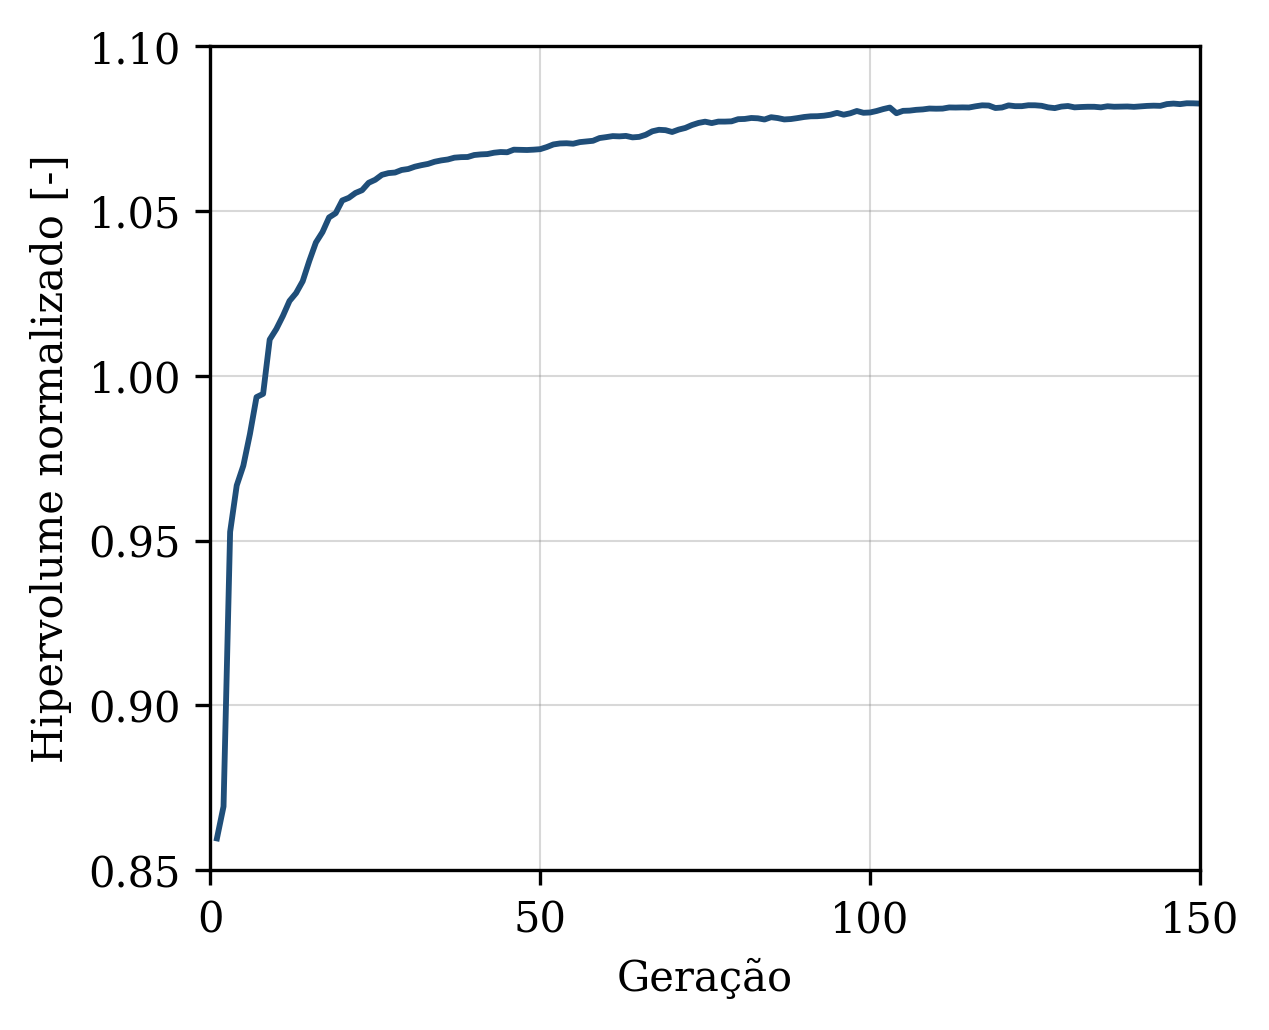
\includegraphics[width=0.7\textwidth]{figuras/convergencia_hv.png}
    \caption{Evolução do hipervolume ao longo das gerações do NSGA-II.}
    \label{fig:convergencia_hv}
\end{figure}

\begin{table}[!ht]
\caption{Hipervolume final, \textit{spacing} e geração de estabilização das vinte células da matriz.\label{tab:hv}}
\begin{threeparttable}
\begin{tabular*}{\columnwidth}{@{\extracolsep\fill}llccc@{\extracolsep\fill}}
\toprule
Célula & $L$ (m) / Classe & $HV$ & \textit{Spacing} & Geração de estabilização \\
\midrule
C-01 & 3{,}0 / D20 & 1{,}103 & 0{,}0195 & 37 \\
C-02 & 3{,}0 / D30 & 1{,}107 & 0{,}0216 & 44 \\
C-03 & 3{,}0 / D40 & 1{,}131 & 0{,}0203 & 43 \\
C-04 & 3{,}0 / D50 & 1{,}140 & 0{,}0187 & 28 \\
C-05 & 3{,}0 / D60 & 1{,}135 & 0{,}0195 & 23 \\
\midrule
C-06 & 4{,}0 / D20 & 1{,}025 & 0{,}0174 & 37 \\
C-07 & 4{,}0 / D30 & 1{,}092 & 0{,}0198 & 34 \\
C-08 & 4{,}0 / D40 & 1{,}124 & 0{,}0197 & 70 \\
C-09 & 4{,}0 / D50 & 1{,}120 & 0{,}0183 & 28 \\
C-10 & 4{,}0 / D60 & 1{,}118 & 0{,}0210 & 30 \\
\midrule
C-11 & 5{,}0 / D20 & 1{,}046 & 0{,}0183 & 60 \\
C-12 & 5{,}0 / D30 & 1{,}067 & 0{,}0169 & 50 \\
\textbf{C-13} & 5{,}0 / D40 & 1{,}083 & 0{,}0162 & 59 \\
C-14 & 5{,}0 / D50 & 1{,}108 & 0{,}0171 & 52 \\
C-15 & 5{,}0 / D60 & 1{,}123 & 0{,}0216 & 39 \\
\midrule
C-16 & 6{,}0 / D20 & 1{,}041 & 0{,}0152 & 51 \\
C-17 & 6{,}0 / D30 & 1{,}052 & 0{,}0192 & 35 \\
C-18 & 6{,}0 / D40 & 1{,}063 & 0{,}0204 & 46 \\
C-19 & 6{,}0 / D50 & 1{,}083 & 0{,}0190 & 46 \\
C-20 & 6{,}0 / D60 & 1{,}105 & 0{,}0233 & 45 \\
\bottomrule
\end{tabular*}
\begin{tablenotes}
\footnotesize
\item Ponto de referência $r_1 = r_2 = 1{,}1$ no espaço objetivo normalizado pelos pontos ideal e nadir de cada execução, o que fixa em 1{,}21 o valor máximo teórico do indicador.
O \textit{spacing} é o desvio padrão das distâncias entre soluções consecutivas da fronteira final, no mesmo espaço normalizado. Valores menores indicam distribuição mais uniforme.
A geração de estabilização é a primeira a partir da qual o hipervolume permanece dentro de 1\% do valor final.
\end{tablenotes}
\end{threeparttable}
\end{table}

A curva da Figura~\ref{fig:convergencia_hv} apresenta o comportamento típico de uma execução bem dimensionada: crescimento acentuado nas primeiras vinte gerações, quando o algoritmo localiza a região viável e ordena a primeira frente, seguido de refinamento assintótico.
Para a célula C-13, o hipervolume atinge 1{,}083 e permanece dentro de 1\% desse valor a partir da geração 59, isto é, em pouco menos de 40\% das 150 gerações executadas.
Estendendo a leitura a toda a matriz, a estabilização ocorre entre as gerações 23 e 70, com média de 43.
A célula mais lenta a convergir, a C-08, estabiliza na geração 70, ainda com folga de 80 gerações.
O valor $N_{gen} = 150$ da Tabela~\ref{tab:nsga2} está, portanto, confirmado a posteriori para todas as células, e não apenas para a de referência, ao custo de um excedente de esforço computacional que se justifica por dispensar o ajuste individual do orçamento de gerações célula a célula.

O hipervolume final varia entre 1{,}025 e 1{,}140, ou seja, entre 85\% e 94\% do máximo teórico, e decresce sistematicamente com o vão dentro de cada classe: as células de 6~m apresentam os menores valores, e as de 3~m os maiores.
Essa tendência não indica pior convergência nos vãos maiores, e sim fronteiras mais curtas no espaço objetivo, pois o intervalo de compromisso entre volume e flecha se estreita quando as restrições se tornam mais severas.
O \textit{spacing} varia pouco em toda a matriz, entre 0{,}0152 e 0{,}0233, com média de 0{,}0191, e não apresenta correlação com o vão ou com a classe.
A leitura conjunta dos dois indicadores é a que importa: a extensão da fronteira, medida pelo hipervolume, depende da severidade do caso, ao passo que a uniformidade da distribuição das soluções, medida pelo \textit{spacing}, é homogênea.
Em outras palavras, o algoritmo entrega fronteiras igualmente bem distribuídas em todas as células, ainda que mais ou menos extensas conforme o caso, o que é a condição necessária para que a Tabela~\ref{tab:resultados_matriz} possa ser comparada linha a linha.

\subsubsection{Análise de sensibilidade global por índices de Sobol}\label{sec:sobol}

Para identificar quais variáveis de projeto mais influenciam a violação de cada restrição sob perturbação, realizou-se uma análise de sensibilidade global pelo método de Sobol \parencite{Sobol2001}, implementado na biblioteca \texttt{UQpy} \parencite{Olivier2020}.
Os índices de efeito total $S_{T_i}$ das cinco variáveis de projeto foram estimados em relação às seis funções limite, a partir de uma amostragem independente de $N = 20\,000$ pontos no domínio de cada variável (Tabela~\ref{tab:intervalos}).

\begin{figure}[!ht]
    \centering
    
\includegraphics[width=0.85\textwidth]{figuras/sobol_heatmap_C13.png}
    \caption{Índices de Sobol de efeito total ($S_{T_i}$) das variáveis de projeto sobre as restrições, célula C-13.}
    \label{fig:sobol}
\end{figure}

\begin{table}[!ht]
\caption{Variável de maior influência ($S_{T_i}$ dominante) por restrição.\label{tab:sobol}}
\begin{threeparttable}
\footnotesize
\setlength{\tabcolsep}{3pt}
\begin{tabular*}{\columnwidth}{@{\extracolsep\fill}lccc@{\extracolsep\fill}}
\toprule
Restrição & Variável dominante & $S_{T_i}$ & Participação \\
\midrule
$g_1$: flexão da longarina & $d$ & 1{,}051 & 96{,}6\% \\
$g_2$: cisalhamento da longarina & $d$ & 1{,}176 & 90{,}4\% \\
$g_3$: flecha da longarina & $d$ & 0{,}999 & 95{,}0\% \\
$g_4$: flexão do tabuleiro & $esp_{long}$ & 13{,}221 & 81{,}2\% \\
$g_5$: espaçamento entre longarinas & $esp_{long}$ & 1{,}003 & 100{,}0\% \\
$g_6$: espaçamento entre peças do tabuleiro & $esp_{tab}$ & 1{,}000 & 100{,}0\% \\
\bottomrule
\end{tabular*}
\begin{tablenotes}
\footnotesize
\item A participação relativa é a fração do somatório dos índices de efeito total das cinco variáveis para aquela restrição, calculada após truncar em zero as estimativas negativas.
Os índices de efeito total são estimados por diferença de variâncias e, por isso, não são limitados ao intervalo $[0,1]$ em respostas fortemente não lineares: o valor de 13{,}221 associado a $g_4$ reflete a não linearidade do arredondamento do número inteiro de peças acomodadas na pista, e não uma participação superior a 100\%.
A leitura correta desses índices é comparativa, isto é, de ordenação entre variáveis, e não absoluta.
\end{tablenotes}
\end{threeparttable}
\end{table}

O resultado confirma a expectativa mecânica para as três restrições da longarina.
O diâmetro $d$ responde por 96{,}6\% da sensibilidade da flexão, 90{,}4\% do cisalhamento e 95{,}0\% da flecha, ao passo que as quatro variáveis restantes somam, em conjunto, menos de 10\% em qualquer uma delas.
O domínio é esperado porque $d$ é a única variável que entra simultaneamente na área, no módulo resistente e no momento de inércia da seção circular (Equações~\eqref{eq:areacirc} a~\eqref{eq:rcirc}), e é ainda mais pronunciado no estado limite de serviço, no qual o momento de inércia varia com $d^4$ enquanto a área, que governa o peso próprio, varia apenas com $d^2$.

A flexão do tabuleiro comporta-se de modo distinto e mais informativo.
Nela, o diâmetro é praticamente irrelevante, com participação de 0{,}3\%, e a variável dominante passa a ser o espaçamento entre longarinas, com 81{,}2\%, seguido pela altura da prancha, com 11{,}5\%, e pela largura, com 6{,}6\%.
A explicação é imediata: o espaçamento entre longarinas é o vão de flexão local da prancha sob a roda do trem tipo, e o momento solicitante cresce com o quadrado desse vão, ao passo que a resistência da prancha cresce apenas com $b_w h^2$.
O espaçamento entre longarinas é, portanto, a variável de acoplamento entre os dois subsistemas da superestrutura: ela não afeta a longarina isoladamente, mas define quanto do carregamento chega a cada uma e qual o vão que o tabuleiro precisa vencer.
As duas últimas restrições são, por construção, funções exclusivas dos respectivos espaçamentos, e a análise as recupera com participação de 100\%, o que serve como verificação de consistência do próprio estimador.

A leitura de engenharia desses índices é a de uma hierarquia de controle de execução.
Duas grandezas concentram praticamente toda a sensibilidade do conjunto: o diâmetro das peças roliças e o espaçamento entre longarinas.
São elas que justificam investimento em controle dimensional rigoroso, o primeiro na etapa de seleção e classificação das toras, com rejeição das peças fora da faixa nominal, e o segundo na etapa de montagem, com gabarito de posicionamento das longarinas.
As dimensões da prancha do tabuleiro, $b_w$ e $h$, e o espaçamento entre peças do tabuleiro, $esp_{tab}$, admitem tolerâncias de execução mais folgadas sem prejuízo mensurável à segurança, uma vez que respondem por parcela reduzida da variabilidade das funções limite.
Essa distinção é relevante em obra vicinal, na qual o controle de qualidade é necessariamente seletivo e precisa ser direcionado ao que efetivamente importa.

\subsubsection{Dispersão das variáveis de projeto ao longo da fronteira}\label{sec:dispersao}

Como complemento aos indicadores de qualidade da fronteira no espaço objetivo, a Figura~\ref{fig:boxplot} caracteriza a diversidade da fronteira no espaço de decisão, apresentando a dispersão de cada variável de projeto entre as soluções não dominadas.

\begin{figure}[!ht]
    \centering
    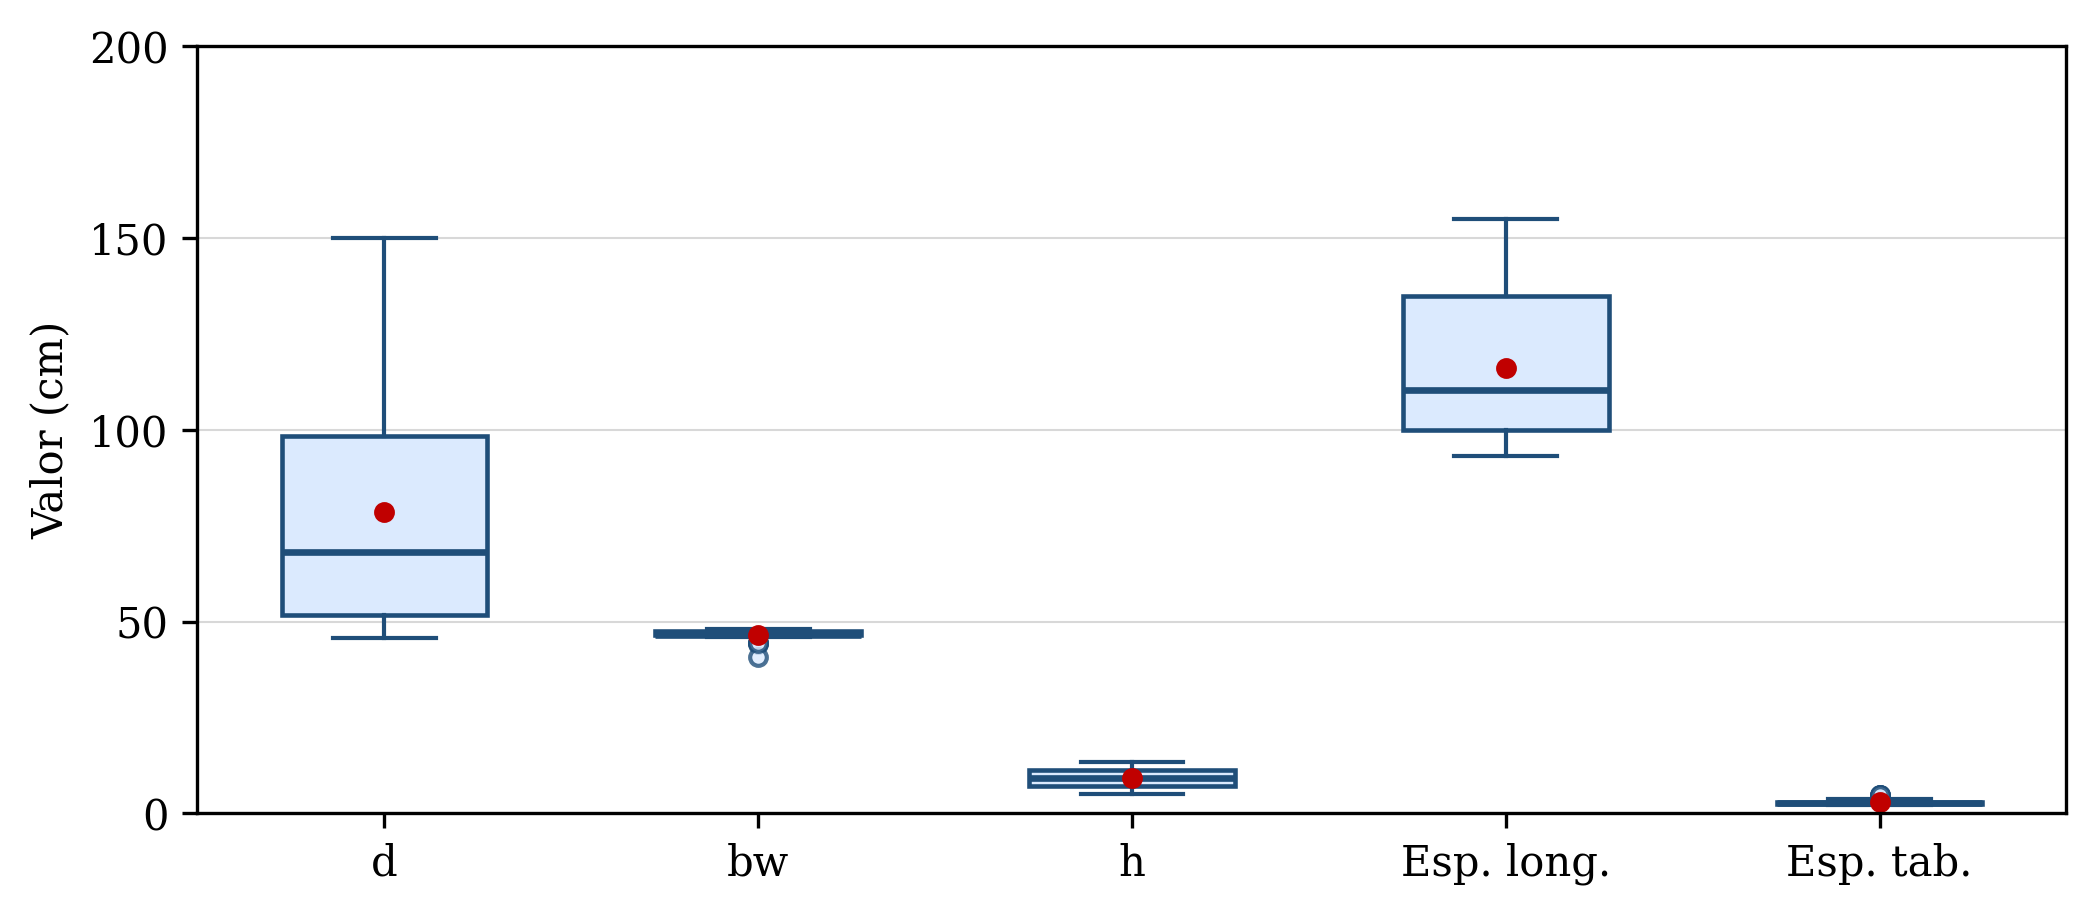
\includegraphics[width=0.75\textwidth]{figuras/boxplot_variaveis_C13.png}
    \caption{Dispersão das variáveis de projeto ao longo da fronteira eficiente da célula C-13.}
    \label{fig:boxplot}
\end{figure}

\begin{table}[!ht]
\caption{Estatística descritiva das variáveis de projeto na fronteira eficiente da célula C-13.\label{tab:estatistica}}
\begin{threeparttable}
\footnotesize
\setlength{\tabcolsep}{3pt}
\begin{tabular*}{\textwidth}{@{\extracolsep{\fill}}lccccccccc@{\extracolsep{\fill}}}
\toprule
Variável & Média & Desv. padrão & CV (\%) & Mínimo & $Q_1$ & Mediana & $Q_3$ & Máximo & Amplitude \\
\midrule
$d$ (cm) & 78{,}58 & 31{,}76 & 40{,}42 & 45{,}71 & 51{,}77 & 68{,}08 & 98{,}39 & 150{,}00 & 104{,}29 \\
$b_w$ (cm) & 46{,}57 & 1{,}24 & 2{,}67 & 40{,}69 & 46{,}44 & 46{,}51 & 47{,}54 & 47{,}93 & 7{,}23 \\
$h$ (cm) & 9{,}17 & 2{,}37 & 25{,}90 & 5{,}09 & 7{,}19 & 9{,}12 & 11{,}20 & 13{,}46 & 8{,}37 \\
$esp_{long}$ (cm) & 116{,}07 & 18{,}76 & 16{,}16 & 93{,}24 & 99{,}82 & 110{,}39 & 134{,}89 & 155{,}04 & 61{,}79 \\
$esp_{tab}$ (cm) & 2{,}92 & 0{,}69 & 23{,}72 & 2{,}19 & 2{,}55 & 2{,}69 & 3{,}08 & 4{,}88 & 2{,}69 \\
\bottomrule
\end{tabular*}
\begin{tablenotes}
\footnotesize
\item Estatísticas calculadas sobre as 50 soluções não dominadas da fronteira final.
A plataforma exporta esta tabela automaticamente.
\end{tablenotes}
\end{threeparttable}
\end{table}

A dispersão é fortemente desigual entre as variáveis, tanto em amplitude absoluta quanto em variação relativa.
O diâmetro da longarina é, com folga, a variável de maior amplitude ao longo da fronteira: 104{,}3~cm de variação, coeficiente de variação de 40{,}4\% e intervalo interquartil de 46{,}6~cm, cobrindo praticamente todo o domínio de busca da Tabela~\ref{tab:intervalos}.
Em seguida vem o espaçamento entre longarinas, com amplitude de 61{,}8~cm, restrita a cerca de um terço da faixa admissível (30 a 200~cm) e com coeficiente de variação comparativamente moderado, 16{,}2\%.
São essas duas variáveis, mesmo assim, que constroem o compromisso entre os dois objetivos: nenhuma outra se aproxima delas em amplitude absoluta.

No extremo oposto, a largura da prancha do tabuleiro é praticamente invariante, com coeficiente de variação de 2{,}7\% e intervalo interquartil de apenas 1{,}1~cm em torno de 46{,}6~cm.
O algoritmo converge para esse valor independentemente do ponto da fronteira escolhido pelo projetista, o que tem consequência prática relevante: $b_w \approx 46{,}5$~cm pode ser fixado a priori no anteprojeto, sem penalidade de desempenho, reduzindo de cinco para quatro a dimensionalidade efetiva da decisão.
As duas variáveis restantes ocupam posições intermediárias em amplitude absoluta, mas exibem coeficiente de variação elevado precisamente por variarem em torno de uma escala pequena: 25{,}9\% para a altura da prancha (8{,}4~cm de amplitude) e 23{,}7\% para o espaçamento entre peças do tabuleiro (2{,}7~cm de amplitude).
Este último merece nota: o valor mínimo observado na fronteira, 2{,}19~cm, está rente ao mínimo admissível de 2~cm, o que mostra que ao menos a extremidade mais econômica da fronteira aproxima as peças do tabuleiro tanto quanto a regra construtiva permite, porque reduzir o vão local de flexão da prancha é a forma mais barata de aliviar a restrição que governa toda a fronteira.

O confronto com a Seção~\ref{sec:sobol} é convergente, e isso reforça a leitura, desde que a dispersão seja lida em amplitude absoluta, e não em coeficiente de variação, métrica que penaliza artificialmente variáveis de escala pequena como o espaçamento entre peças do tabuleiro.
As duas variáveis de maior sensibilidade são exatamente as duas de maior amplitude absoluta na fronteira, e cada uma comanda um subsistema: o diâmetro responde por 90 a 97\% da sensibilidade das três verificações da longarina e é a variável de maior amplitude na fronteira. O espaçamento entre longarinas responde por 81{,}2\% da sensibilidade da flexão do tabuleiro e é a segunda de maior amplitude.
Percorrer a fronteira consiste, portanto, em ajustar simultaneamente esses dois parâmetros, um por subsistema.
As três variáveis restantes, que reúnem baixa sensibilidade e amplitude absoluta reduzida, comportam-se como parâmetros construtivos e não como variáveis de decisão. Isso sugere que um procedimento de anteprojeto simplificado poderia fixá-las e otimizar apenas $d$ e $esp_{long}$ sem perda relevante de qualidade.

\subsection{Varredura paramétrica: efeito do vão e da classe de resistência}\label{sec:varredura}

Esta seção reporta o resultado das vinte células da matriz.
Para cada célula, extraiu-se da fronteira eficiente a solução de menor volume de madeira, por ser a de interesse imediato para o anteprojeto, e registraram-se as dimensões correspondentes, o volume total, a flecha adimensional e a verificação governante.
Os resultados consolidados constam da Tabela~\ref{tab:resultados_matriz}.

\begin{table}[!ht]
\caption{Resultados consolidados da varredura paramétrica: solução de menor volume de madeira em cada célula da matriz.\label{tab:resultados_matriz}}
\begin{threeparttable}
\footnotesize
\setlength{\tabcolsep}{3pt}
\begin{tabular*}{\textwidth}{@{\extracolsep{\fill}}llrrrrrrrrl@{\extracolsep{\fill}}}
\toprule
Célula & $L$ (m) / Classe & $d$ & $b_w$ & $h$ & $esp_{long}$ & $esp_{tab}$ & $V_{\mathrm{total}}$ & $\delta_{\mathrm{tot}}/(L/350)$ & $g_{\max}$ & Verificação \\
 & & (cm) & (cm) & (cm) & (cm) & (cm) & (m\textsuperscript{3}) & & & governante \\
\midrule
C-01 & 3{,}0 / D20 & 39{,}65 & 5{,}14 & 5{,}00 & 50{,}35 & 5{,}00 & 2{,}519 & 0{,}1325 & $-0{,}0030$ & Flexão long. \\
C-02 & 3{,}0 / D30 & 34{,}66 & 33{,}72 & 5{,}00 & 57{,}63 & 4{,}78 & 2{,}195 & 0{,}1912 & $-0{,}0032$ & Flexão long. \\
C-03 & 3{,}0 / D40 & 31{,}52 & 38{,}78 & 6{,}62 & 69{,}61 & 4{,}29 & 1{,}969 & 0{,}2375 & $-0{,}0012$ & Flexão long. \\
C-04 & 3{,}0 / D50 & 30{,}18 & 16{,}64 & 5{,}04 & 51{,}86 & 4{,}99 & 1{,}829 & 0{,}2435 & $-0{,}0023$ & Flexão tab. \\
C-05 & 3{,}0 / D60 & 30{,}00 & 34{,}77 & 5{,}00 & 64{,}99 & 4{,}30 & 1{,}762 & 0{,}2178 & $-0{,}0166$ & Flexão tab. \\
\midrule
C-06 & 4{,}0 / D20 & 50{,}19 & 28{,}82 & 5{,}03 & 62{,}56 & 4{,}88 & 4{,}711 & 0{,}1629 & $-0{,}0007$ & Flexão tab. \\
C-07 & 4{,}0 / D30 & 43{,}90 & 46{,}89 & 5{,}01 & 53{,}87 & 4{,}44 & 3{,}849 & 0{,}2324 & $-0{,}0130$ & Flexão long. \\
C-08 & 4{,}0 / D40 & 40{,}10 & 46{,}28 & 12{,}43 & 194{,}97 & 4{,}75 & 3{,}574 & 0{,}3152 & $-0{,}0011$ & Flexão tab. \\
C-09 & 4{,}0 / D50 & 36{,}97 & 40{,}46 & 5{,}05 & 73{,}59 & 3{,}93 & 2{,}964 & 0{,}3381 & $-0{,}0075$ & Flexão long. \\
C-10 & 4{,}0 / D60 & 34{,}73 & 40{,}73 & 5{,}00 & 69{,}57 & 3{,}18 & 2{,}705 & 0{,}3710 & $-0{,}0003$ & Flexão long. \\
\midrule
C-11 & 5{,}0 / D20 & 57{,}88 & 47{,}68 & 15{,}30 & 199{,}91 & 2{,}52 & 7{,}120 & 0{,}2014 & $-0{,}0043$ & Flexão long. \\
C-12 & 5{,}0 / D30 & 50{,}59 & 47{,}51 & 13{,}24 & 193{,}41 & 2{,}05 & 5{,}761 & 0{,}2907 & $-0{,}0033$ & Flexão long. \\
\textbf{C-13} & 5{,}0 / D40 & 45{,}71 & 46{,}51 & 7{,}51 & 103{,}58 & 2{,}26 & 4{,}829 & 0{,}3355 & $-0{,}0000$ & Flexão tab. \\
C-14 & 5{,}0 / D50 & 42{,}71 & 52{,}39 & 10{,}40 & 195{,}63 & 3{,}71 & 4{,}339 & 0{,}4226 & $-0{,}0028$ & Flexão long. \\
C-15 & 5{,}0 / D60 & 40{,}19 & 47{,}63 & 6{,}55 & 108{,}12 & 2{,}25 & 3{,}892 & 0{,}4244 & $-0{,}0005$ & Flexão tab. \\
\midrule
C-16 & 6{,}0 / D20 & 63{,}81 & 51{,}85 & 13{,}94 & 116{,}46 & 2{,}77 & 9{,}219 & 0{,}2250 & $-0{,}0010$ & Flexão tab. \\
C-17 & 6{,}0 / D30 & 55{,}78 & 52{,}04 & 12{,}30 & 118{,}55 & 4{,}48 & 7{,}462 & 0{,}3248 & $-0{,}0014$ & Flexão long. \\
C-18 & 6{,}0 / D40 & 50{,}70 & 53{,}90 & 10{,}73 & 177{,}56 & 3{,}75 & 6{,}317 & 0{,}3976 & $-0{,}0006$ & Flexão long. \\
C-19 & 6{,}0 / D50 & 47{,}13 & 51{,}84 & 10{,}04 & 156{,}13 & 2{,}68 & 5{,}641 & 0{,}4716 & $-0{,}0011$ & Flexão tab. \\
C-20 & 6{,}0 / D60 & 44{,}45 & 54{,}03 & 9{,}15 & 192{,}19 & 2{,}95 & 5{,}088 & 0{,}5139 & $-0{,}0020$ & Flexão tab. \\
\bottomrule
\end{tabular*}
\begin{tablenotes}
\footnotesize
\item Todas as células com $\rho = 5\%$ e os parâmetros de algoritmo da Tabela~\ref{tab:nsga2}.
A coluna ``Verificação governante'' registra a restrição com maior valor de $g_j$ entre $g_1$ e $g_4$ na solução reportada, isto é, a que está mais próxima do limite normativo, e $g_{\max}$ é o valor correspondente.
\item As vinte células apresentaram solução viável, de modo que não há linha ``inviável'' a registrar.
A hipótese de inviabilidade nas classes de menor resistência sob os maiores vãos, plausível a priori, não se confirmou: a célula C-16 ($L = 6{,}0$~m, D20), a mais desfavorável da matriz, converge para uma solução viável com longarinas de 63{,}8~cm de diâmetro.
\end{tablenotes}
\end{threeparttable}
\end{table}

\paragraph{Efeito do vão.} O consumo de madeira cresce de forma mais que proporcional ao vão em todas as classes, como esperado, mas o expoente da lei de potência $V \propto L^{n}$ ajustada às quatro observações de cada classe depende da classe: $n = 1{,}89$ para D20, 1{,}78 para D30, 1{,}67 para D40, 1{,}64 para D50 e 1{,}54 para D60, com coeficientes de determinação superiores a 0{,}988 em todos os casos.
Em termos absolutos, passar de 3{,}0 para 6{,}0~m multiplica o consumo por 3{,}7 na classe D20 e por 2{,}9 na classe D60.
O expoente maior nas classes de menor resistência é a assinatura do acoplamento entre peso próprio e desempenho: na madeira de baixa resistência a seção precisa crescer mais para atender à flexão, o que aumenta o peso próprio, o que por sua vez exige seção ainda maior.
Nas classes altas essa realimentação é mais fraca, e a curva de consumo aproxima-se de um crescimento pouco mais que linear.

\paragraph{Efeito da classe de resistência.} A redução de volume ao subir de classe é acentuada nos vãos de 4~m ou mais e bem menor no vão de 3~m.
Ao passar de D20 para D60, o consumo cai 42{,}6\% no vão de 4~m, 45{,}3\% no de 5~m e 44{,}8\% no de 6~m, mas apenas 30{,}0\% no vão de 3~m.
A explicação está na Tabela~\ref{tab:resultados_matriz}: nas células C-04 e C-05, ambas de 3~m, o diâmetro converge para praticamente 30~cm, o limite inferior do domínio de busca da Tabela~\ref{tab:intervalos}; já a célula C-03, com diâmetro discretamente acima do piso (31{,}5~cm), opera saturada estruturalmente, com apenas 0{,}1\% de folga na flexão da longarina ($g_{\max} = -0{,}0012$).
A partir da classe D40, portanto, o dimensionamento no vão de 3~m deixa de ter folga relevante, seja por estar junto ao limite normativo, seja por estar junto ao mínimo comercial das peças roliças: as três células operam com $g_{\max}$ entre $-0{,}0012$ e $-0{,}0166$, contra folgas de $-0{,}20$ a $-0{,}47$ nas mesmas classes nos vãos maiores.
O resultado tem leitura prática direta: em vãos de cerca de 3~m não há vantagem em especificar madeira acima da classe D40, pois a estrutura já opera junto ao limite normativo ou ao limite dimensional das toras disponíveis, e a escolha entre D40, D50 e D60 deve recair sobre durabilidade e disponibilidade local, não sobre resistência.

Nos vãos maiores, o primeiro degrau de classe é sistematicamente o mais rentável.
Passar de D20 para D30 reduz o consumo em 18{,}3\% no vão de 4~m, 19{,}1\% no de 5~m e 19{,}1\% no de 6~m, ao passo que os degraus seguintes rendem entre 7{,}1\% e 17{,}1\%, sem decaimento estritamente monotônico.
A causa do achatamento é a compensação apontada na formulação do problema: entre D20 e D60 a resistência característica à flexão triplica e o módulo de elasticidade quase dobra, mas a densidade também dobra, de 500 para 1000~kg/m\textsuperscript{3}, e o acréscimo de peso próprio consome parte do ganho de resistência.
O ganho não chega a se anular nem a se inverter dentro da faixa estudada, de modo que não existe, a rigor, uma classe ótima no sentido de um mínimo interior.
Do ponto de vista de anteprojeto, a recomendação que decorre da matriz é que o esforço de especificação se concentre em garantir pelo menos a classe D30 nos vãos de 4~m ou mais, degrau que sozinho responde por cerca de 40\% de toda a economia disponível entre D20 e D60, e que a busca por classes superiores só se justifique quando a madeira de classe alta estiver disponível sem sobrecusto relevante.

A matriz é integralmente monotônica, o que é a verificação de consistência esperada: dentro de cada classe o volume cresce com o vão, e dentro de cada vão decresce da classe D20 para a D60, sem uma única inversão nas vinte células.

\paragraph{Verificação governante.} A última coluna da Tabela~\ref{tab:resultados_matriz} revela um mapa distinto do que a intuição sugeriria.
Nem a flecha da longarina nem o cisalhamento governam qualquer uma das vinte células: as vinte são governadas por flexão, onze pela flexão da longarina e nove pela flexão do tabuleiro.
As duas verificações alternam-se ao longo da matriz sem um padrão nítido em vão ou classe, o que é coerente com o que a Seção~\ref{sec:fronteira_ref} mostrou para a célula de referência: as duas flexões tornam-se ativas quase simultaneamente na solução econômica, e qual delas fica marginalmente à frente depende de detalhes do arredondamento do número inteiro de peças acomodadas na pista.

A consequência prática é relevante e vai na direção oposta da expectativa corrente.
Em pontes de madeira roliça nesta faixa de vãos, sob o TB-240, a propriedade do material que importa é a resistência à flexão em toda a matriz, e não a rigidez: o estado limite de serviço de deslocamento, comumente tido como determinante em estruturas de madeira, permanece com folga de pelo menos 48\% em todas as células, conforme o valor máximo de $\delta_{\mathrm{tot}}/(L/350)$ igual a 0{,}514 registrado na célula C-20.
Igualmente relevante é a ausência do cisalhamento, tradicionalmente citado como crítico em peças roliças curtas: a área da seção circular cresce com $d^2$ enquanto a solicitação de cortante independe do diâmetro, de modo que essa verificação nunca se aproxima do limite.
A transição de resistência para rigidez, que caracterizaria vãos maiores, situa-se portanto fora da faixa de 3 a 6~m e só deve ser esperada em extensões superiores, o que delimita com precisão o campo de validade dos ábacos da seção seguinte.
Cabe notar, por fim, que o tabuleiro governa nove das vinte células e permanece a restrição ativa em toda a fronteira da célula de referência: ele não é um elemento secundário do dimensionamento, e merece no anteprojeto a mesma atenção dedicada às longarinas.

\subsection{Ábacos de anteprojeto}\label{sec:abacos}

Os resultados da Tabela~\ref{tab:resultados_matriz} foram convertidos em ábacos de consulta direta, destinados ao uso do projetista na etapa de concepção, antes de qualquer processamento computacional.
A Figura~\ref{fig:abaco_volume} apresenta o volume total de madeira em função do vão, com uma curva por classe de resistência. A Figura~\ref{fig:abaco_volume_m2} normaliza esse volume pela área de tabuleiro, permitindo comparação direta entre vãos. Já a Figura~\ref{fig:abaco_diametro} fornece o diâmetro de longarina requerido, que é a informação de aquisição mais imediata para o construtor.

\begin{figure}[!ht]
    \centering
    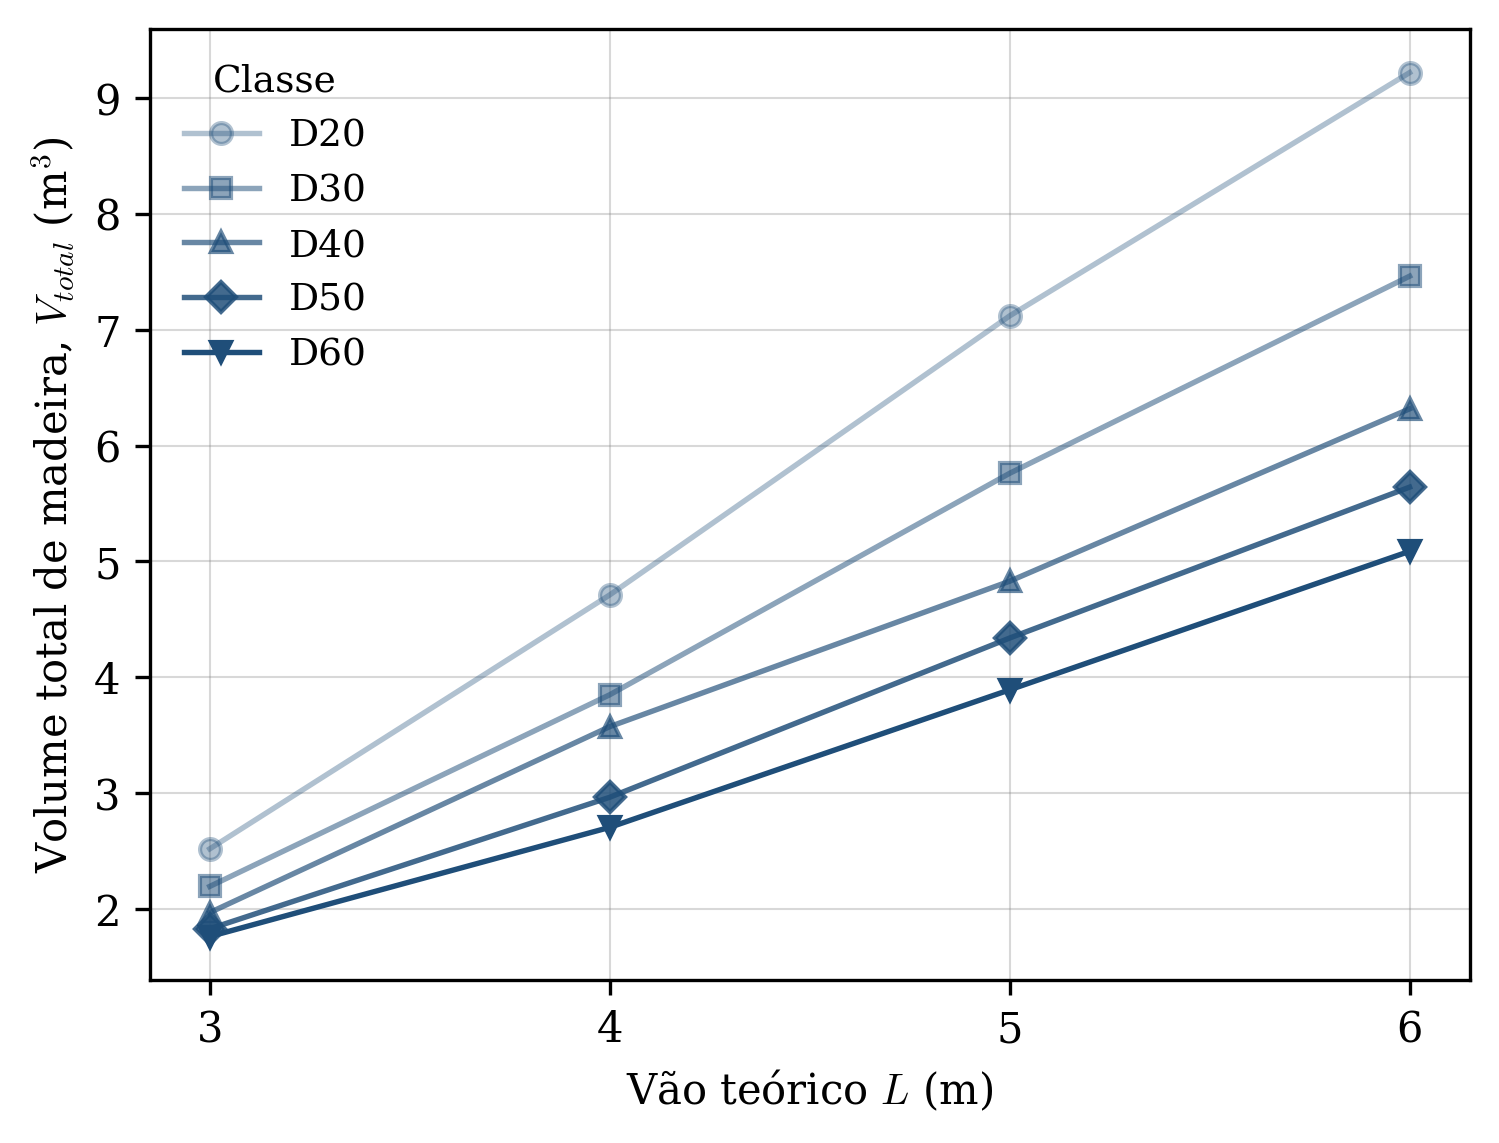
\includegraphics[width=0.7\textwidth]{figuras/abaco_volume_vs_vao.png}
    \caption{Volume total de madeira em função do vão teórico, por classe de resistência.}
    \label{fig:abaco_volume}
\end{figure}

\begin{figure}[!ht]
    \centering
    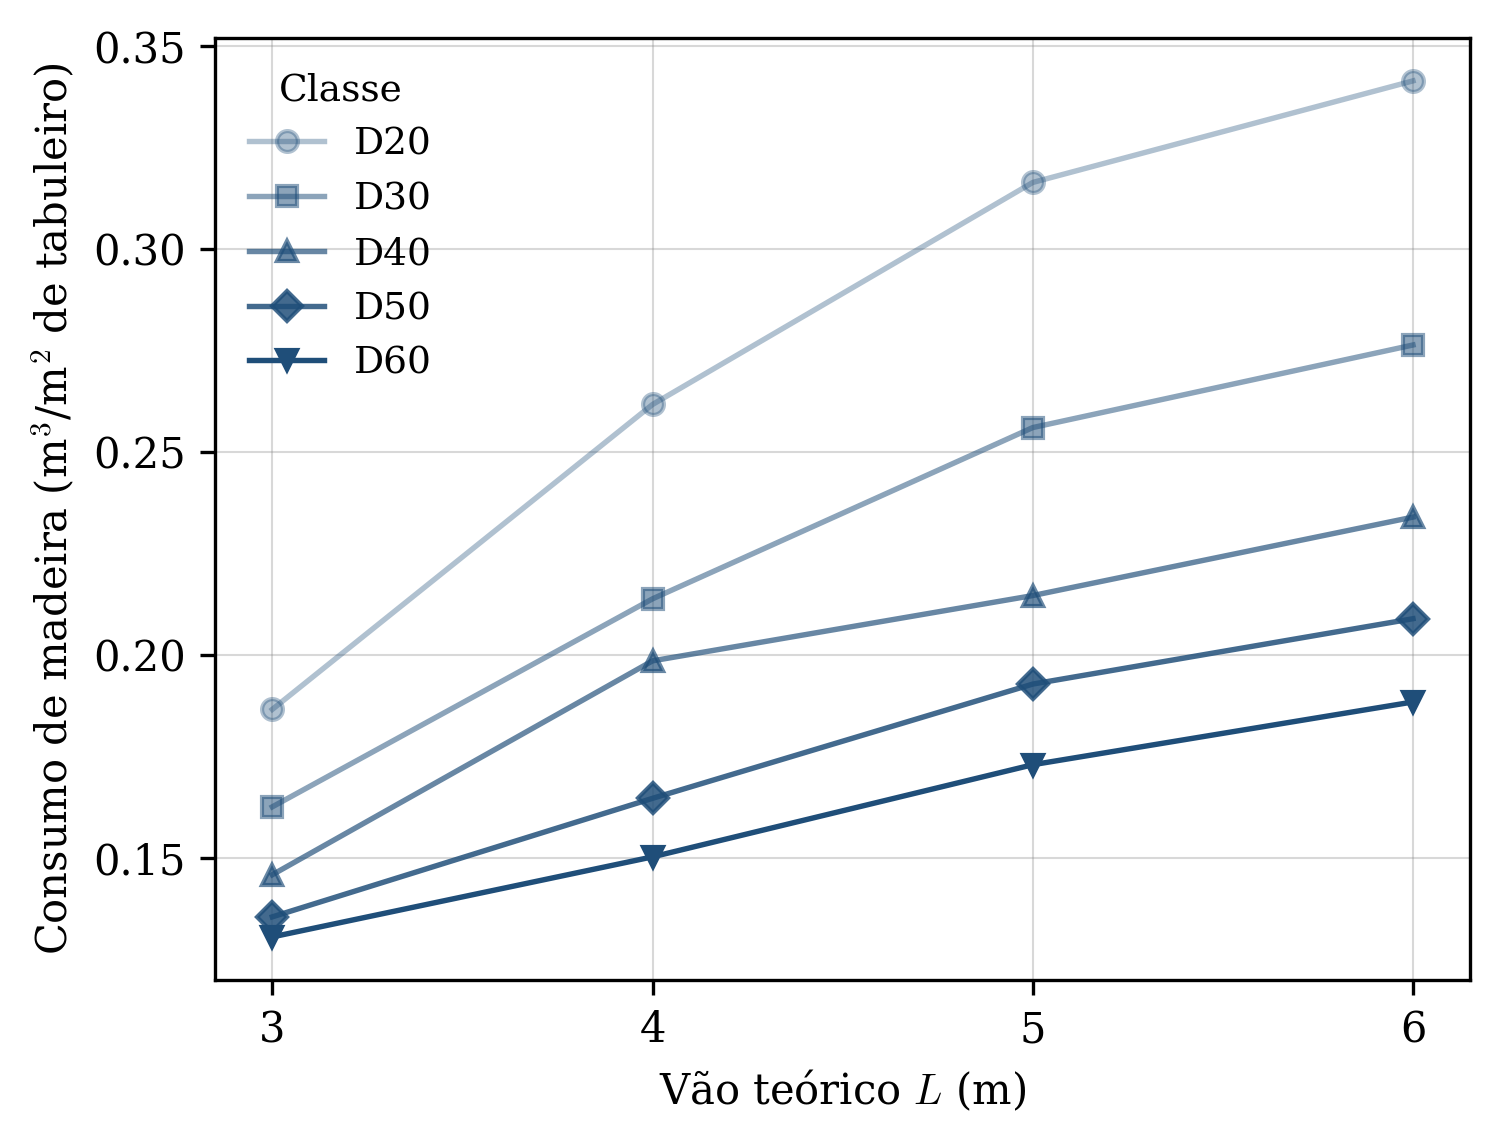
\includegraphics[width=0.7\textwidth]{figuras/abaco_volume_por_m2.png}
    \caption{Consumo de madeira por metro quadrado de tabuleiro, em função do vão teórico, por classe de resistência.}
    \label{fig:abaco_volume_m2}
\end{figure}

\begin{figure}[!ht]
    \centering
    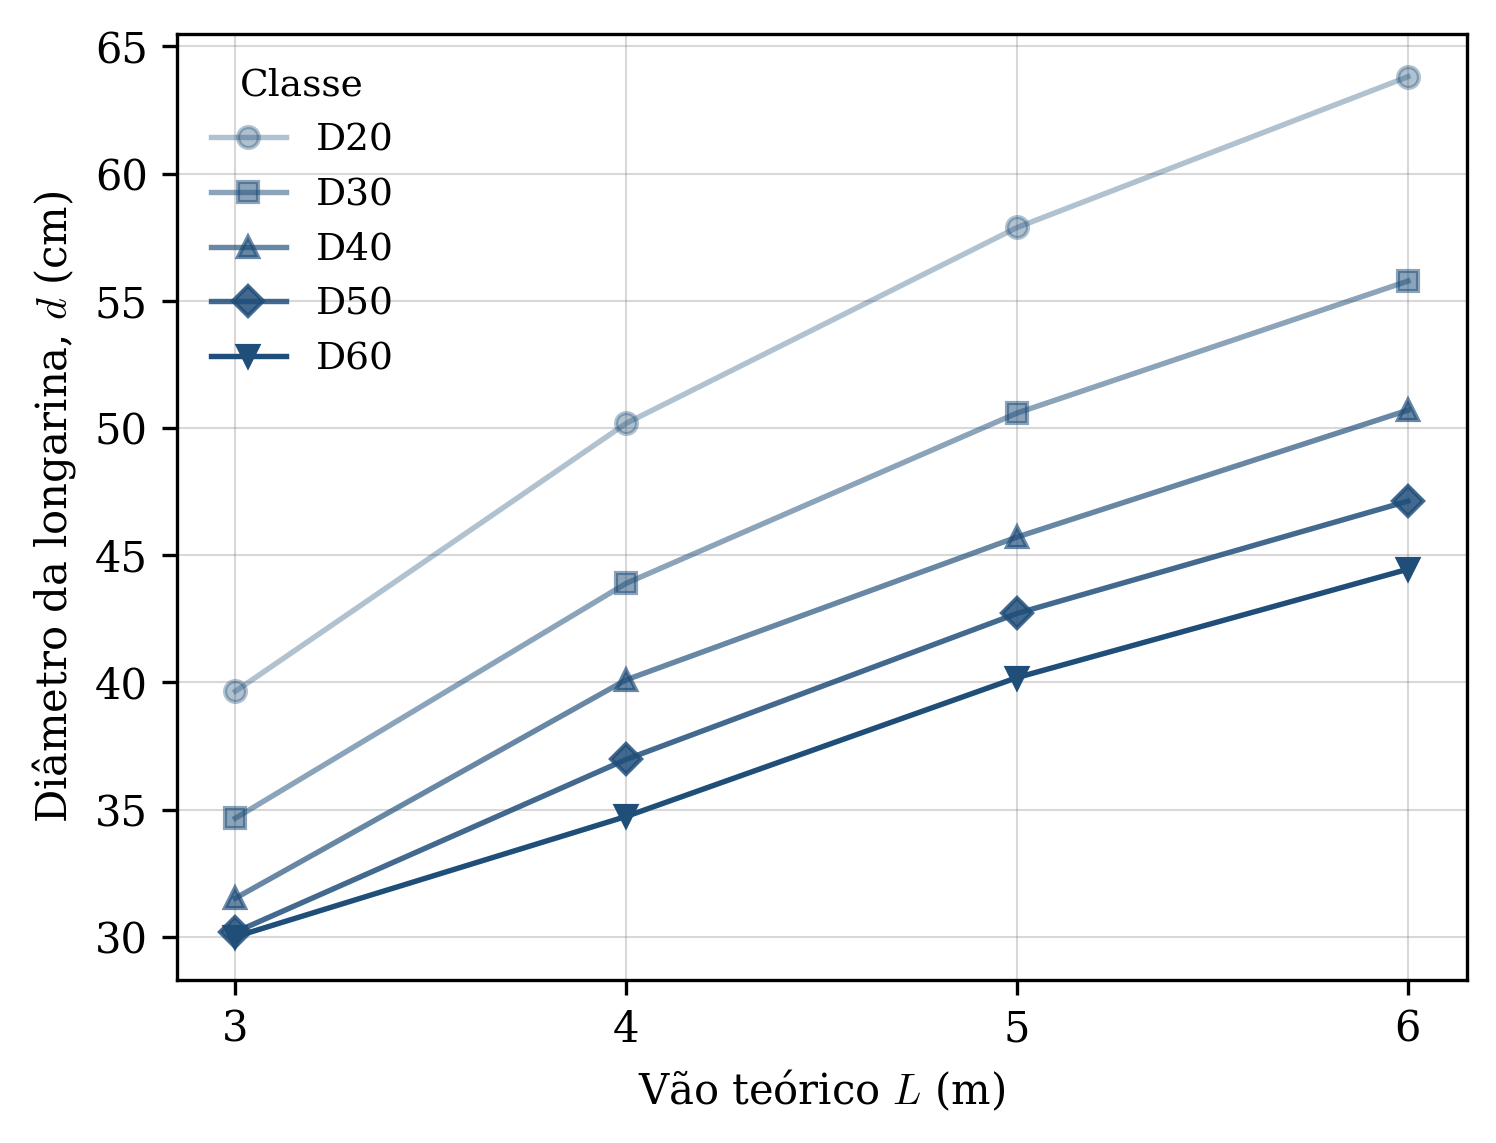
\includegraphics[width=0.7\textwidth]{figuras/abaco_diametro_vs_vao.png}
    \caption{Diâmetro de longarina requerido em função do vão teórico, por classe de resistência.}
    \label{fig:abaco_diametro}
\end{figure}

O uso dos ábacos segue um roteiro de quatro passos.
Primeiro, entra-se com o vão teórico a vencer no eixo horizontal, arredondado para cima até um dos quatro valores tabelados.
Segundo, escolhe-se a curva correspondente à classe de resistência da madeira efetivamente disponível na região da obra, e não à classe desejada, uma vez que a disponibilidade local é a restrição real em estradas vicinais.
Terceiro, lê-se na Figura~\ref{fig:abaco_volume} o volume total esperado, que serve à estimativa de custo e de logística de transporte, e na Figura~\ref{fig:abaco_diametro} o diâmetro de longarina requerido, que é a informação de aquisição imediata, pois define a bitola das toras a encomendar.
A Figura~\ref{fig:abaco_volume_m2} permite ainda comparar a eficiência entre vãos, ao normalizar o consumo pela área de tabuleiro, e mostra que o consumo unitário varia de 0{,}13~m\textsuperscript{3}/m\textsuperscript{2} no vão de 3~m com D60 a 0{,}34~m\textsuperscript{3}/m\textsuperscript{2} no vão de 6~m com D20.
Quarto, entram-se esses valores na plataforma como ponto de partida para a verificação detalhada, no mesmo formato demonstrado passo a passo no Apêndice~\ref{ap:demonstracao}.

As condições de validade dos ábacos são exatamente as da Tabela~\ref{tab:parametros} e devem ser verificadas antes de qualquer leitura: pista simples de 4{,}5~m de largura, trem tipo TB-240 com carga por roda de 40~kN e carga de multidão de 4~kPa, classe de umidade 3, classe de carregamento de curta duração, coeficiente de fluência de 0{,}80, madeira natural de florestas nativas enquadrada nas classes da Tabela~\ref{tab:classes_madeira} e desvio de robustez de 5\%.
Fora dessas condições, e em particular para larguras de pista diferentes ou para vãos superiores a 6~m, as curvas não se aplicam, já que a formulação do momento devido à carga móvel muda de expressão e a hierarquia entre as verificações governantes pode se alterar, conforme discutido na Seção~\ref{sec:varredura}.

Cabe o alerta de que os ábacos não substituem a verificação estrutural: eles a antecipam.
Os valores lidos correspondem à solução de menor volume da fronteira eficiente de cada célula, isto é, ao dimensionamento mais econômico que ainda atende a todas as restrições sob a avaliação robusta, e por construção operam muito próximo do limite normativo em pelo menos uma verificação, conforme os valores de $g_{\max}$ da Tabela~\ref{tab:resultados_matriz}.
Qualquer alteração de premissa em relação à Tabela~\ref{tab:parametros}, por menor que seja, pode tornar essa solução inviável.
O papel dos ábacos é eliminar o arbitramento inicial de seções na etapa de concepção e permitir a estimativa de quantitativos antes de qualquer processamento, transferindo para a plataforma a responsabilidade pela verificação definitiva.
